\documentclass{article}
\usepackage[polish]{babel}
\usepackage[T1]{fontenc}
\usepackage{float}
\usepackage{subcaption}
\usepackage{caption}
\usepackage[a4paper,top=2cm,bottom=2cm,left=3cm,right=3cm,marginparwidth=1.75cm]{geometry}
\usepackage{amsmath}
\usepackage{graphicx}
\usepackage{hyperref}

\title{Uruchomienie algorytmów wyznaczania trasy dla sieci drogowej}
\author{Adrian Fabisiewicz (328935), Julia Gomulska (328936)}

\begin{document}
\maketitle

\section{Opis ćwiczenia}

Celem ćwiczenia było uruchomienie algorytmów wyznaczania trasy dla sieci drogowej. W ramach ćwiczenia zaimplementowano algorytmy Djikstry oraz A*. Stworzony program odczytuje sieć drogową z wybranego źródła oraz uruchamia wyznaczanie trasy pomiędzy dwoma punktami, uwzględniając kierunkowość dróg. Następnie zwraca trasę najkrótszą oraz najszybszą. Program zintegrowano z oprogramowaniem GIS - ArcGIS Pro, dzięki czemu użytkownik ma możliwość ręcznego wybrania punktów początkowego i końcowego na mapie. Zaimplementowano również rozszerzenie, pozwalające na wyznaczenie zasięgu obszaru, do którego można dojechać z danego punktu w określonym przez użytkownika czasie.

\section{Środowisko pracy oraz wykorzystane dane}
Ćwiczenie zostało wykonane w języku Python z wykorzystaniem biblioteki ArcPy. Do kontroli wersji korzystano z systemu Git. Danymi wejściowymi były dane BDOT dla Torunia i powiatu toruńskiego, udostępnione przez prowadzącego.

\section{Opracowane algorytmy}
Algorytm został opracowany na podstawie ...

\section{Integracja z GIS}
Utworzony program został zintegrowany ze środowiskiem ESRI ArcGIS Pro. Narzędzie w oprogramowaniu pozwala na wyznaczenie trasy pomiędzy dwoma punktami na mapie. 
Punkty są pobierane z wybranej dwupunktowej warstwy zawierającej punkt początkowy i punkt końcowy, bądź zaznaczane kliknięciem. Należy również wybrać warstwę zawierającą sieć drogową, po której ma zostać wyznaczona trasa. Użytkownik ma możliwość wyboru, czy chce wyznaczyć trasę najkrótszą, czy najszybszą, czy obie z nich. Po uruchomieniu narzędzia, program wyznacza wybrane trasy i dodaje je do mapy. W logach programu zwracane są informacje o czasie najszybszej trasy i długości najkrótszej trasy. Interfejs narzędzia został zaprezentowany na rysunku 1.

\begin{figure}[H]
    \centering
    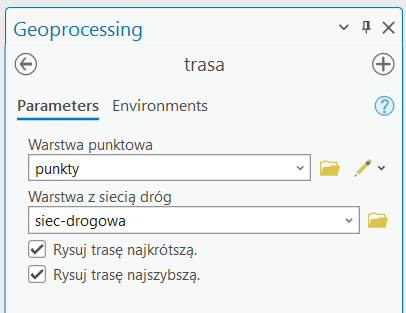
\includegraphics[width=0.5\textwidth]{img/narzedzie-interfejs-trasa.png}
    \caption{Interfejs narzędzia do wyznaczenia trasy}
\end{figure}

\section{Przykłady działania algorytmu wyznaczającego trasy}
\subsection{Przykład 1: Dworzec Główny - Galeria Copernicus}
\begin{figure}[H]
    \centering
    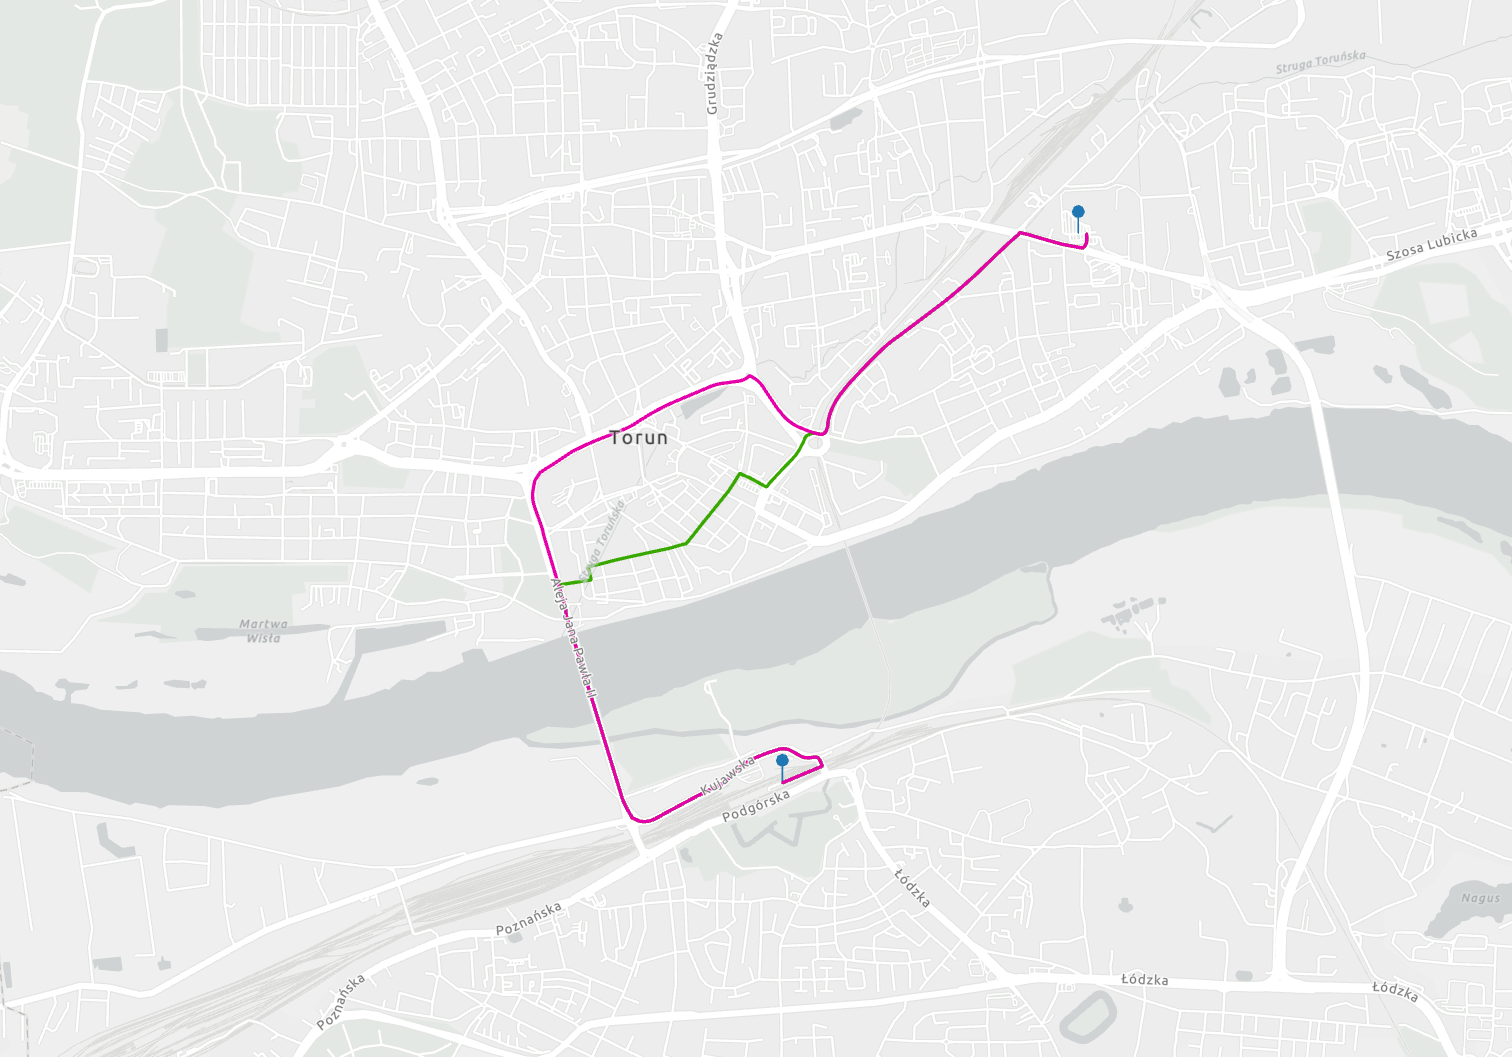
\includegraphics[width=1\textwidth]{img/glowny-copernicus.png}
    \caption{Trasy wyznaczone przez stworzone narzędzie (na zielono - trasa najkrótsza, na różowo - najszybsza)}
\end{figure}

\begin{figure}[H]
    \centering
    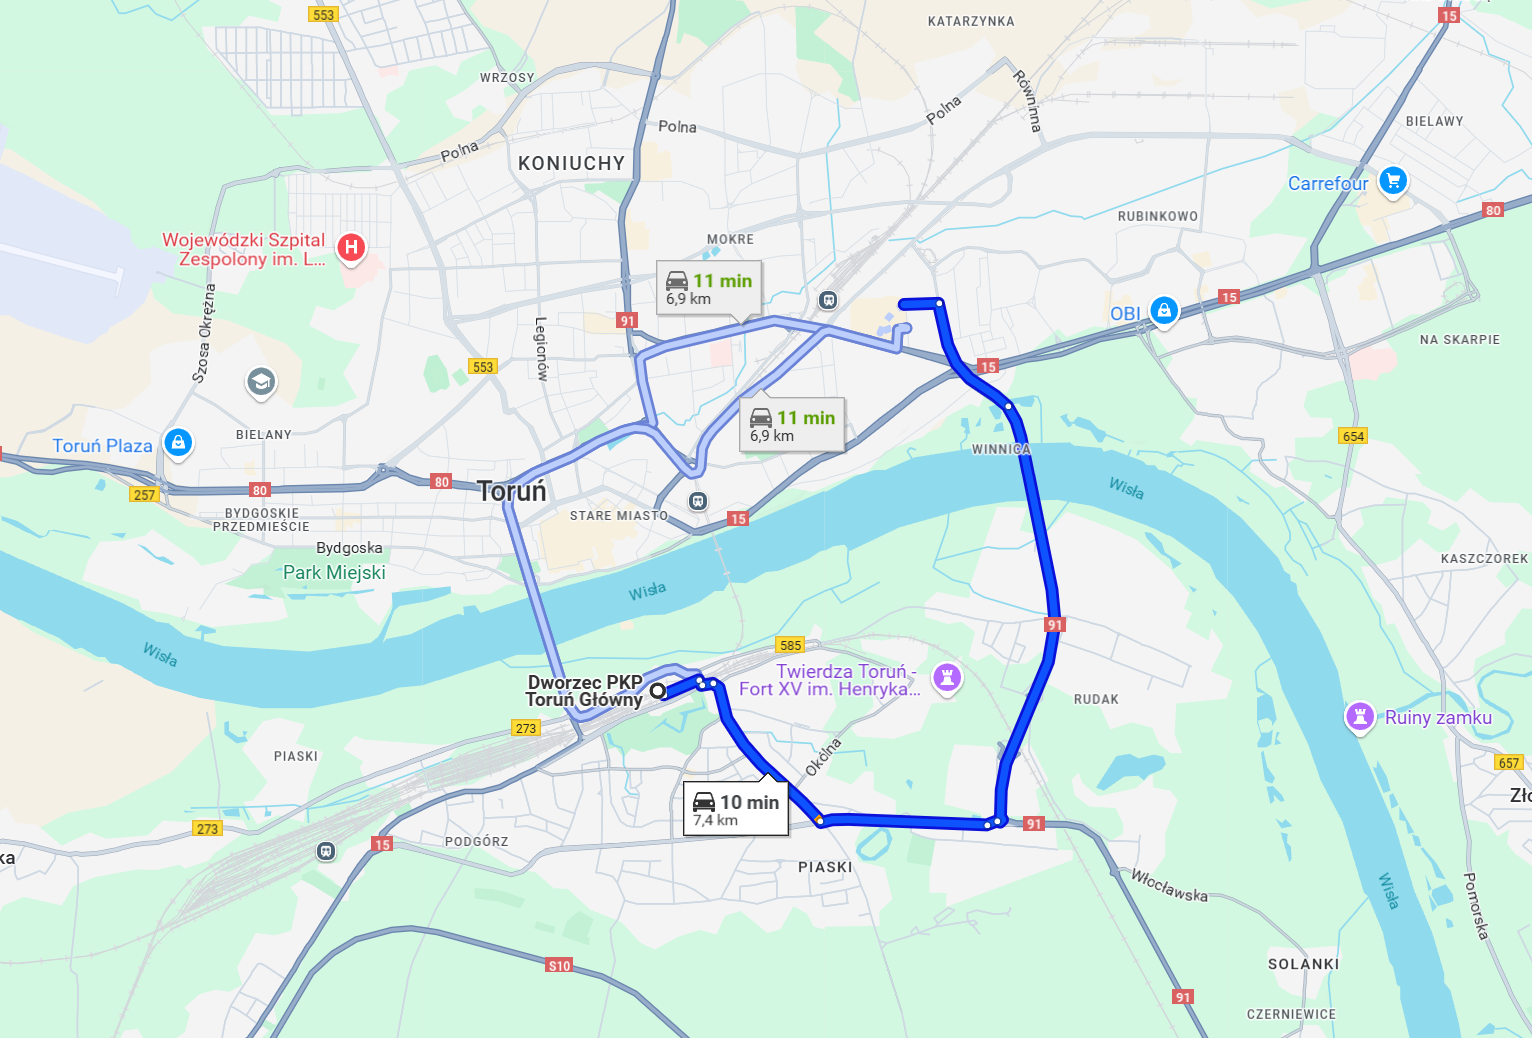
\includegraphics[width=1\textwidth]{img/glowny-copernicus-google.png}
    \caption{Trasy proponowane przez Google Maps}
\end{figure}

\subsection{Przykład 2: Motoarena - ROD Zielone Wzgórze}
\begin{figure}[H]
    \centering
    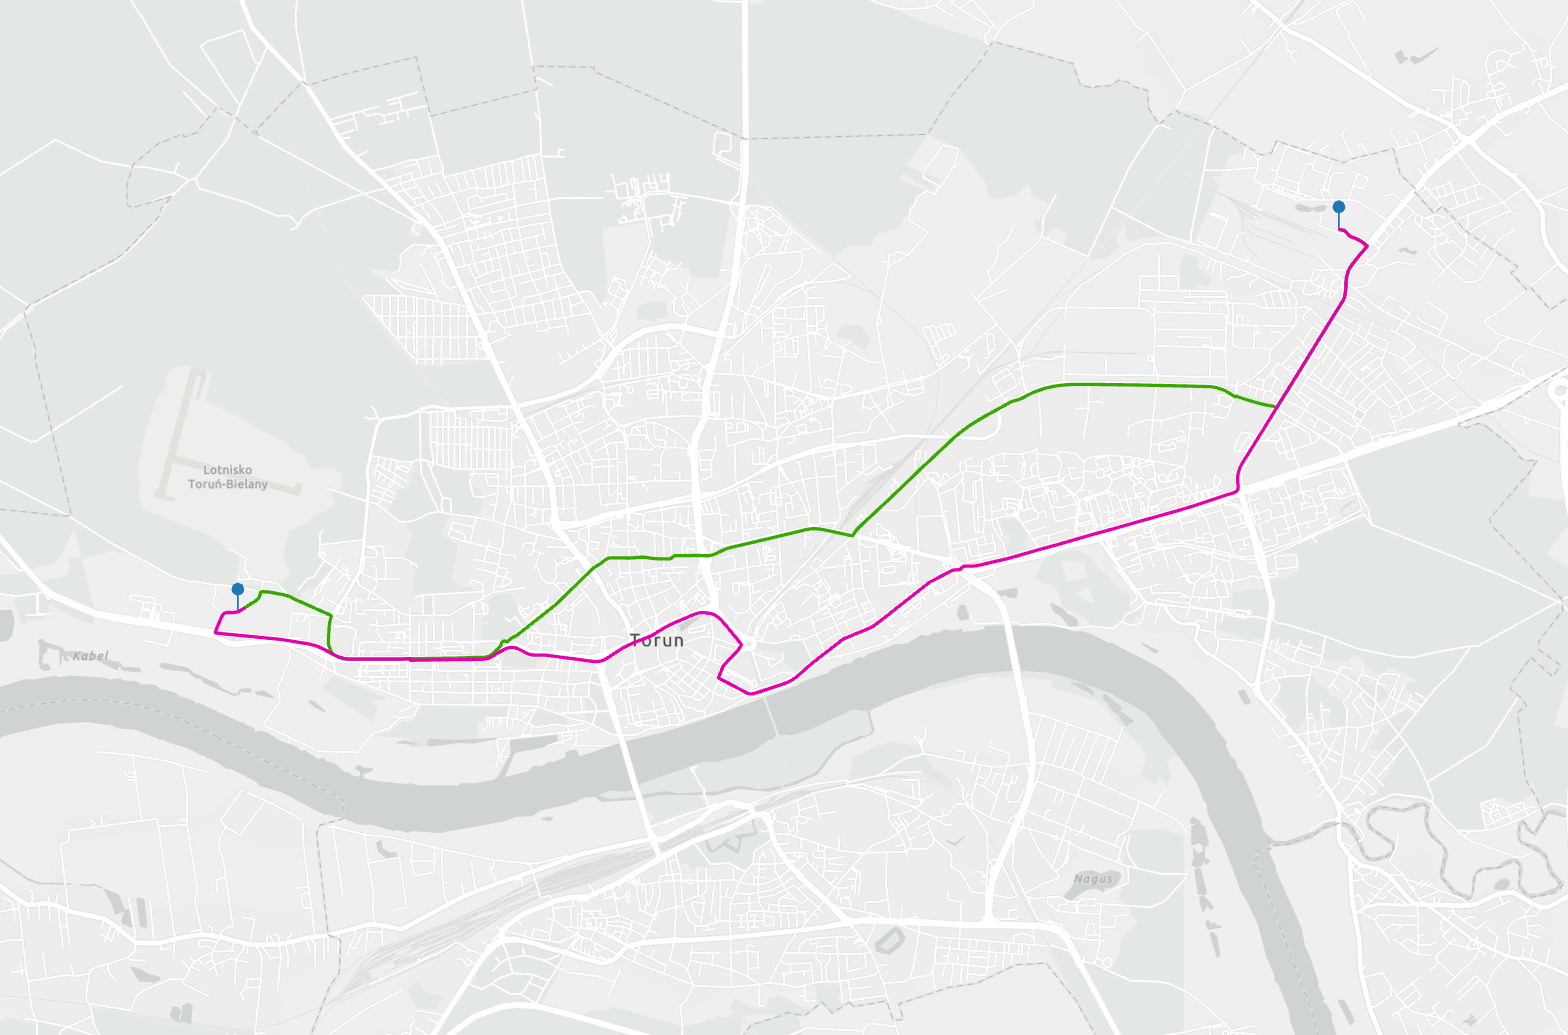
\includegraphics[width=1\textwidth]{img/motoarena-rod.png}
    \caption{Trasy wyznaczone przez stworzone narzędzie (na zielono - trasa najkrótsza, na różowo - najszybsza)}
\end{figure}

\begin{figure}[H]
    \centering
    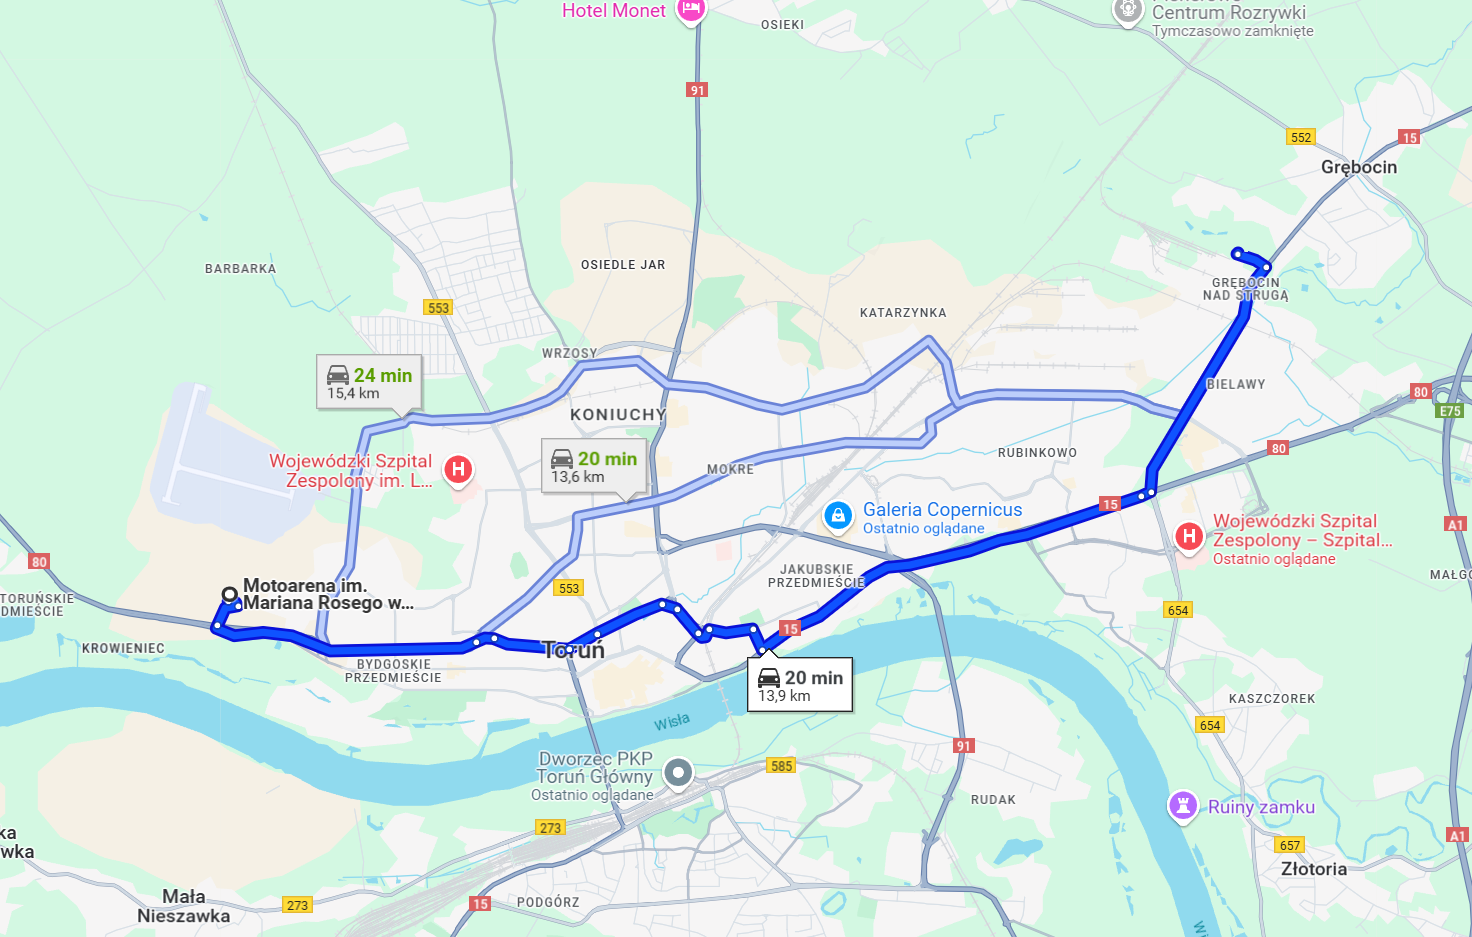
\includegraphics[width=1\textwidth]{img/motoarena-rod-google.png}
    \caption{Trasy proponowane przez Google Maps}
\end{figure}

\section{Zasięg}
\subsection{Integracja z GIS}
Program do wyznaczania zasięgu również zintegrowano ze środowiskiem ArcGIS Pro. Użytkownik ma możliwość wybrania punktu początkowego na mapie, a następnie określenia czasu, w jakim chce dojechać do punktów z zasięgu. Program zwraca obszar, do którego można dojechać w wybranym czasie. Interfejs narzędzia został zaprezentowany na rysunku 6.

\begin{figure}[H]
    \centering
    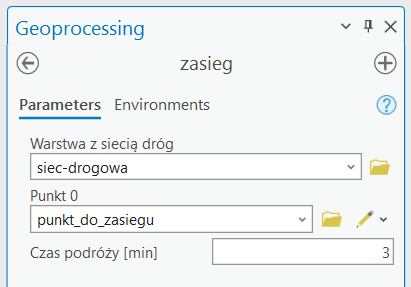
\includegraphics[width=0.5\textwidth]{img/narzedzie-interfejs-zasieg.png}
    \caption{ Interfejs narzędzia do wyznaczania zasięgu}
\end{figure}

\subsection{Przykłady działania}
\subsubsection{Przykład 1: Rynek Staromiejski}
\begin{figure}[H]
    \centering
    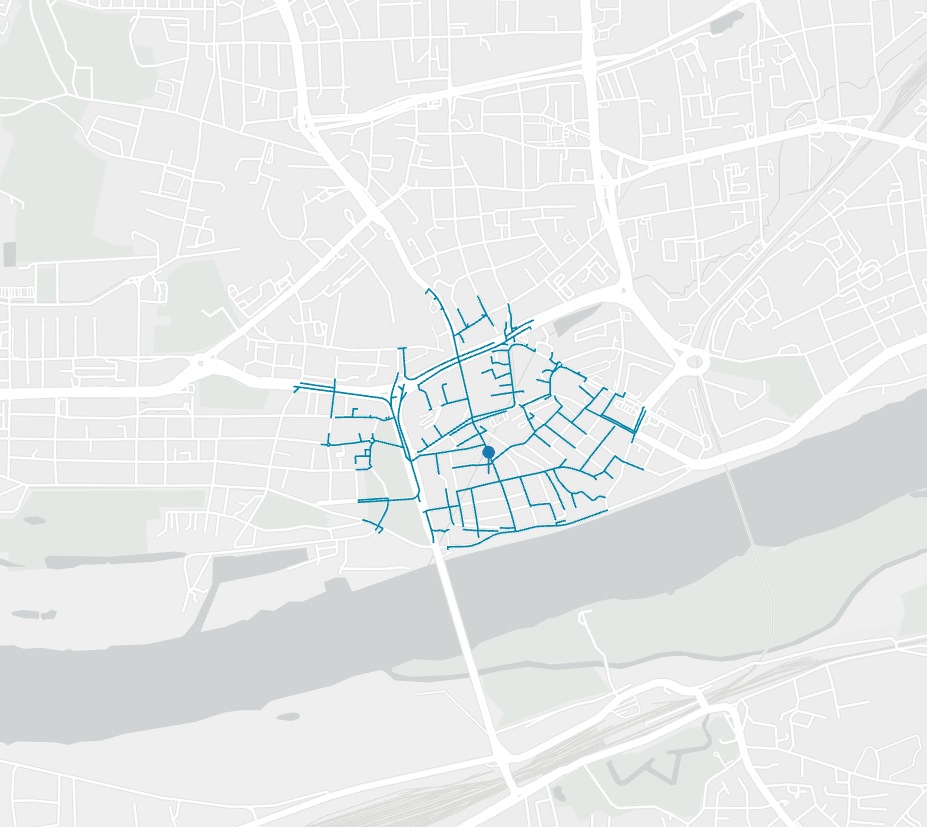
\includegraphics[width=1\textwidth]{img/rynek-2-min.png}
    \caption{Trasy możliwe do pokonania w 2 minuty z punktu startowego na Rynku Staromiejskim}
\end{figure}

\subsubsection{Przykład 2: Biblioteka Uniwersytecka}
\begin{figure}[H]
    \centering
    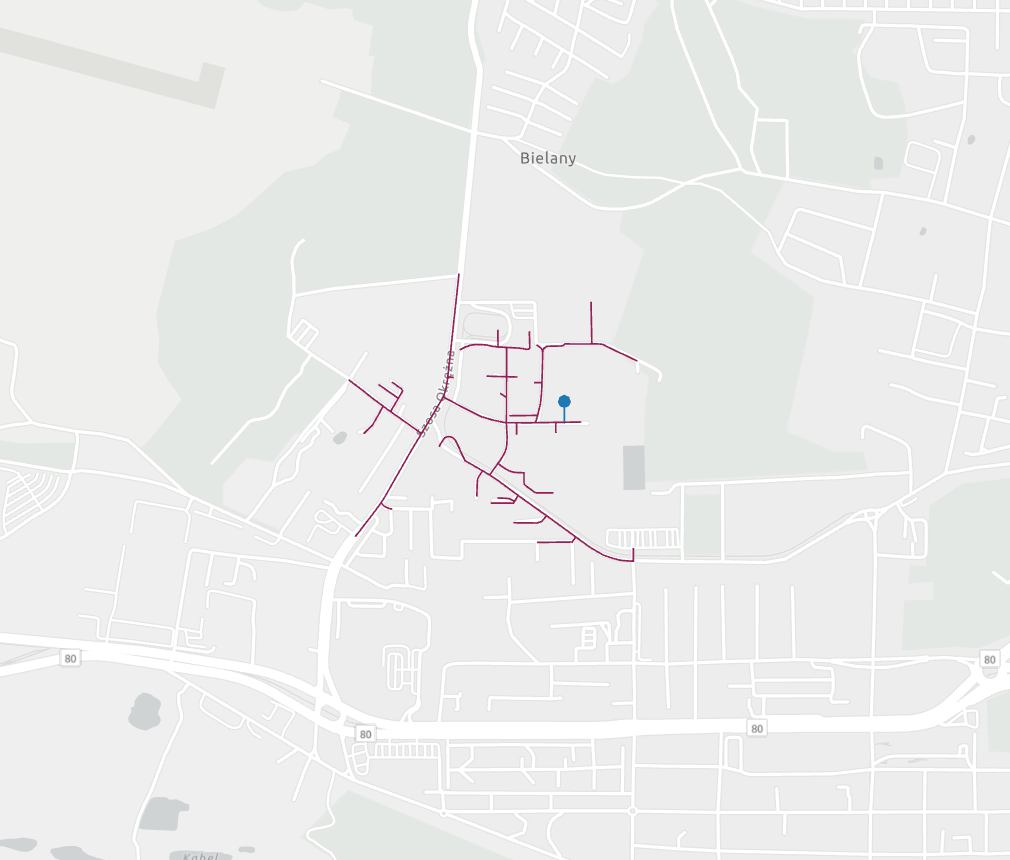
\includegraphics[width=1\textwidth]{img/umk-1-min.png}
    \caption{Trasy możliwe do pokonania w 1 minutę z punktu startowego przy Bibliotece Uniwesyteckiej}
\end{figure}

\section{Wnioski}
\section{Referencje}
\end{document}
